%% ===========================================================================
%%  Latent-space driven active learning of MLIPs for Li|LLZO interfaces
%%  A0 portrait poster -- IISc blue/gold styling, after the BS thesis deck
%%  Build:  tectonic poster_iisc.tex
%%  Scope:  core methodology + energy/force accuracy + data efficiency only
%% ===========================================================================
\documentclass[final]{beamer}
\usepackage[orientation=portrait,size=a0,scale=0.88]{beamerposter}
\usetheme{default}

\usepackage[T1]{fontenc}
\usepackage[utf8]{inputenc}
\usepackage{lmodern}
\usepackage{amsmath,amssymb}
\usepackage{graphicx}
\usepackage{booktabs}
\usepackage{colortbl}
\usepackage{xcolor}
\usepackage{tikz}
\usetikzlibrary{arrows.meta,positioning,shapes.geometric,fit,calc,backgrounds}
\usepackage{array}
\usepackage{multirow}
\usepackage{microtype}
\graphicspath{{figs/}{./}}

%% -- Colours (from the thesis deck) ----------------------------------------
\definecolor{iiscblue}{RGB}{0,54,110}
\definecolor{iiscgold}{RGB}{180,135,0}
\definecolor{lightblue}{RGB}{220,235,250}
\definecolor{lightgold}{RGB}{255,248,210}
\definecolor{wincolor}{RGB}{20,100,40}
\definecolor{winbg}{RGB}{220,245,225}
\definecolor{badcolor}{RGB}{150,20,20}
\definecolor{badbg}{RGB}{250,220,220}
\definecolor{neutgray}{RGB}{90,90,90}

\usecolortheme[named=iiscblue]{structure}
\setbeamertemplate{navigation symbols}{}

\setbeamercolor{block title}{bg=iiscblue,fg=white}
\setbeamercolor{block body}{bg=lightblue,fg=black}
\setbeamercolor{block title alerted}{bg=badcolor,fg=white}
\setbeamercolor{block body alerted}{bg=badbg,fg=black}
\setbeamercolor{block title example}{bg=wincolor,fg=white}
\setbeamercolor{block body example}{bg=winbg,fg=black}

\setbeamerfont{block title}{size=\large,series=\bfseries}
\setbeamerfont{block body}{size=\normalsize}

\setbeamertemplate{itemize item}{\color{iiscblue}$\blacktriangleright$}
\setbeamertemplate{itemize subitem}{\color{iiscgold}$\triangleright$}
\setbeamertemplate{enumerate item}{\color{iiscblue}\insertenumlabel.}

%% block = blue title bar + gold rule + tinted body
\newlength{\blkskip}\setlength{\blkskip}{0.7ex}
\makeatletter
\define@key{beamerframe}{t}[true]{}
\setbeamertemplate{block begin}{%
  \vskip\blkskip
  \begin{beamercolorbox}[wd=\textwidth,leftskip=0.7em,rightskip=0.7em,sep=0.55ex]{block title}%
    \usebeamerfont{block title}\insertblocktitle%
  \end{beamercolorbox}%
  \nointerlineskip
  \noindent{\color{iiscgold}\rule{\textwidth}{0.10cm}}\par
  \nointerlineskip
  \begin{beamercolorbox}[leftskip=0.7em,rightskip=0.7em,vmode]{block body}%
    \vskip1.0ex\justifying
}
\setbeamertemplate{block end}{\vskip1.0ex\end{beamercolorbox}\vskip0.3ex}

\setbeamertemplate{block alerted begin}{%
  \vskip\blkskip
  \begin{beamercolorbox}[wd=\textwidth,leftskip=0.7em,rightskip=0.7em,sep=0.55ex]{block title alerted}%
    \usebeamerfont{block title}\insertblocktitle%
  \end{beamercolorbox}%
  \nointerlineskip
  \begin{beamercolorbox}[leftskip=0.7em,rightskip=0.7em,vmode]{block body alerted}%
    \vskip1.0ex
}
\setbeamertemplate{block alerted end}{\vskip1.0ex\end{beamercolorbox}\vskip0.3ex}

\setbeamertemplate{block example begin}{%
  \vskip\blkskip
  \begin{beamercolorbox}[wd=\textwidth,leftskip=0.7em,rightskip=0.7em,sep=0.55ex]{block title example}%
    \usebeamerfont{block title}\insertblocktitle%
  \end{beamercolorbox}%
  \nointerlineskip
  \begin{beamercolorbox}[leftskip=0.7em,rightskip=0.7em,vmode]{block body example}%
    \vskip1.0ex
}
\setbeamertemplate{block example end}{\vskip1.0ex\end{beamercolorbox}\vskip0.3ex}
\makeatother

\usepackage{ragged2e}

%% -- headline ---------------------------------------------------------------
\setbeamertemplate{headline}{%
  \begin{beamercolorbox}[wd=\paperwidth,ht=0.3cm,dp=0cm]{}%
    \hspace*{0pt}\color{iiscgold}\rule{\paperwidth}{0.3cm}%
  \end{beamercolorbox}
  \nointerlineskip
  \begin{beamercolorbox}[wd=\paperwidth,sep=1.3cm,center]{}%
    \color{iiscblue}
    {\fontsize{64}{74}\selectfont\bfseries
     Latent-Space Driven Active Learning of MLIPs\par
     \vskip0.18em
     for Solid Electrolyte--Electrode Interfaces\par}
    \vskip0.55cm
    {\fontsize{34}{40}\selectfont\bfseries\color{iiscgold}
     Application to Li\,$|$\,LLZO Interfaces at DFT-FE Scale\par}
    \vskip0.7cm
    {\fontsize{30}{36}\selectfont\color{black}
     Mehul Darak \quad\textbullet\quad Rajdeep Boral \quad\textbullet\quad
     Kartick Ramakrishnan \quad\textbullet\quad Phani Motamarri
     \quad\textbullet\quad G.~P.~Das\par}
    \vskip0.35cm
    {\fontsize{26}{32}\selectfont\color{neutgray}
     Department of Computational and Data Sciences, Indian Institute of
     Science, Bengaluru \quad\textbullet\quad TCG CREST, Kolkata\par}
  \end{beamercolorbox}
  \nointerlineskip
  \begin{beamercolorbox}[wd=\paperwidth,ht=0.22cm,dp=0cm]{}%
    \hspace*{0pt}\color{iiscblue}\rule{\paperwidth}{0.22cm}%
  \end{beamercolorbox}
  \vskip0.9cm
}
\setbeamertemplate{footline}{}

%% -- shorthands -------------------------------------------------------------
\newcommand{\wintext}[1]{\textcolor{wincolor}{\textbf{#1}}}
\newcommand{\badtext}[1]{\textcolor{badcolor}{\textbf{#1}}}
\newcommand{\goldtext}[1]{\textcolor{iiscgold}{\textbf{#1}}}
\newcommand{\LLZO}{Li$_7$La$_3$Zr$_2$O$_{12}$}
\newcommand{\figcap}[1]{\par\vspace{0.3em}{\small\textcolor{neutgray}{#1}}}

\begin{document}
\begin{frame}[t]{}
\begin{columns}[t]

%% ======================= COLUMN 1 =======================================
\begin{column}{0.465\paperwidth}

\begin{block}{The interface decides the battery}
Solid-state batteries live or die at the Li-metal\,$|$\,electrolyte interface.
Resolving that chemistry demands molecular dynamics on \textbf{hundreds to
thousands of atoms} --- precisely the regime machine-learned interatomic
potentials were built for.
\vskip0.5em
\begin{itemize}
  \item \LLZO\ against Li metal is \textbf{the} prototypical case: a metal and a
        complex oxide, strong chemical and structural mismatch, and the
        interface that limits every garnet cell.
  \item One supercell is \textbf{420--1378 atoms}; orientation, termination and
        Li-site disorder open a configuration space no direct-DFT campaign can
        reach.
\end{itemize}
\vskip0.4em
\begin{center}\large
\goldtext{We deliver DFT-level accuracy across that whole space --- for 108
labels --- and it is \emph{DFT-FE} that makes it possible.}
\end{center}
\end{block}

\begin{block}{The opening foundation models leave at interfaces}
Foundation MLIPs are trained overwhelmingly on near-equilibrium \emph{bulk}.
Interfaces sit outside that distribution, and the signature is
\badtext{PES softening}: forces underestimated exactly where the physics lives.
\textbf{That gap is the opportunity.}
\vskip0.6em
\begin{columns}[t]
\begin{column}{0.47\textwidth}
\begin{alertblock}{Foundation model, as shipped}
\centering
\begin{tabular}{lr}
\toprule
force RMSE      & \badtext{121.2 meV/\AA} \\
worst component & \badtext{792 meV/\AA}   \\
\bottomrule
\end{tabular}
\end{alertblock}
\end{column}
\begin{column}{0.47\textwidth}
\begin{exampleblock}{After our campaign (it6)}
\centering
\begin{tabular}{lr}
\toprule
force RMSE      & \wintext{72.4 meV/\AA} \\
worst component & \wintext{485 meV/\AA}  \\
\bottomrule
\end{tabular}
\end{exampleblock}
\end{column}
\end{columns}
\vskip0.5em
\begin{center}\large
\wintext{$-$40\% force error.} \wintext{$-$39\% on the worst component anywhere.}
\end{center}
\vskip0.3em
Three ingredients, each doing one job --- and one of them is the enabler:
\goldtext{DFT-FE} produces open-boundary, large-cell labels \textbf{no other
reference method can supply}, \goldtext{latent-space active learning} decides
which of them are worth computing, and \goldtext{LoRA} absorbs them while the
pretrained chemistry stays intact.
\end{block}

\begin{block}{A closed loop that learns what to label}
\centering
\resizebox{0.99\textwidth}{!}{%
\begin{tikzpicture}[x=1cm,y=1cm,>=Stealth,
  bx/.style={draw=iiscblue,very thick,rounded corners=4pt,fill=lightblue,
             text width=3.0cm,minimum height=1.3cm,align=center,
             font=\bfseries\small},
  gx/.style={draw=iiscgold,very thick,rounded corners=4pt,fill=lightgold,
             text width=3.0cm,minimum height=1.3cm,align=center,
             font=\bfseries\small}]
  \node[bx](slabs) at (0,0)      {Interface\\construction};
  \node[bx](md)    at (4.6,0)    {MD sampling\\(NVT)};
  \node[bx](filt)  at (9.2,0)    {Physicality\\filter};
  \node[bx](emb)   at (13.8,0)   {Latent\\extraction};
  \node[gx](fps)   at (18.4,0)   {FPS seeded\\on train set};
  \node[bx](dft)   at (23.0,0)   {DFT-FE\\labelling};
  \node[gx](lora)  at (18.4,-3.4){LoRA\\fine-tuning};

  \foreach \i/\j in {slabs/md,md/filt,filt/emb,emb/fps,fps/dft}{
    \draw[->,very thick,color=iiscblue](\i)--(\j);}
  \draw[->,very thick,color=iiscblue](dft.south) |- (lora.east);
  \draw[thick,dashed,color=iiscgold](lora.west) -- (4.6,-3.4) -- (4.6,-0.9);
  \draw[->,thick,dashed,color=iiscgold](4.6,-0.9) -- (md.south);

  \node[font=\scriptsize,text=neutgray,align=center] at (0,-1.5)
    {3 Li facets\\5 LLZO terms.};
  \node[font=\scriptsize,text=neutgray,align=center] at (9.2,-1.5)
    {keeps the pool clean};
  \node[font=\scriptsize,text=neutgray,align=center] at (13.8,-1.5)
    {256-d\\mean-pooled};
  \node[font=\scriptsize,text=neutgray,align=center] at (23.0,-1.5)
    {420--1378 atoms\\open $z$};
  \node[font=\scriptsize,text=neutgray,align=center,anchor=west] at (20.6,-4.15)
    {rank 5, $<$1\% params};
  \node[font=\scriptsize\itshape,text=iiscgold,align=center] at (4.6,-4.25)
    {the improved model drives the next round};
  \begin{scope}[on background layer]
    \draw[dashed,very thick,color=iiscgold,rounded corners=6pt]
      (2.3,1.6) rectangle (25.2,-4.75);
    \node[font=\small\bfseries,text=iiscgold] at (13.0,2.05)
      {seven rounds, it0 $\rightarrow$ it6};
  \end{scope}
\end{tikzpicture}}
\figcap{Each round samples with the current model, keeps the physical frames,
embeds them in the model's \emph{own} latent space, selects by farthest-point
sampling seeded on everything already labelled, labels with DFT-FE, and
re-fine-tunes --- a better model samples better configurations, which select
better labels.}
\end{block}

\begin{block}{Selection in the model's own latent space}
Every candidate passes through the \textbf{current} model; the rotationally
invariant ($\ell=0$) scalars of the final interaction block give
$\mathbf{z}_i\in\mathbb{R}^{256}$ per atom, mean-pooled to one vector per
structure, $\mathbf{Z}_S=\frac{1}{N_S}\sum_i\mathbf{z}_i$. Distance in this
space is \textbf{the model's own measure of chemical difference}.
\vskip0.5em
\begin{columns}[t]
\begin{column}{0.50\textwidth}
Farthest-point sampling, \textbf{seeded on the existing training set}
$\mathcal{S}$:
\begin{equation*}
k^{*}=\operatorname*{arg\,max}_{k\in\mathcal{P}}\;
\min_{s\in\mathcal{S}}\lVert \mathbf{Z}_k-\mathbf{Z}_s\rVert_2
\end{equation*}
so a near-duplicate of a labelled structure \wintext{can never be picked} ---
de-duplication is \textbf{guaranteed by construction}, not enforced by a
threshold anyone has to tune.
\end{column}
\begin{column}{0.46\textwidth}
\begin{exampleblock}{Coverage, measured exactly}
\begin{equation*}
\delta_k=\min_{s\in\mathcal{S}}\lVert \mathbf{Z}_k-\mathbf{Z}_s\rVert_2,
\qquad \rho=\max_k \delta_k
\end{equation*}
\begin{equation*}
C(d)=\tfrac{1}{|\mathcal{P}|}\bigl|\{k:\delta_k\le d\}\bigr|
\end{equation*}
A \textbf{principled stopping rule}: stop when the worst-covered candidate
falls inside the $d_{99}$ radius. No guesswork about when a round is done.
\end{exampleblock}
\end{column}
\end{columns}
\vskip0.6em
\begin{columns}[t]
\begin{column}{0.52\textwidth}
\centering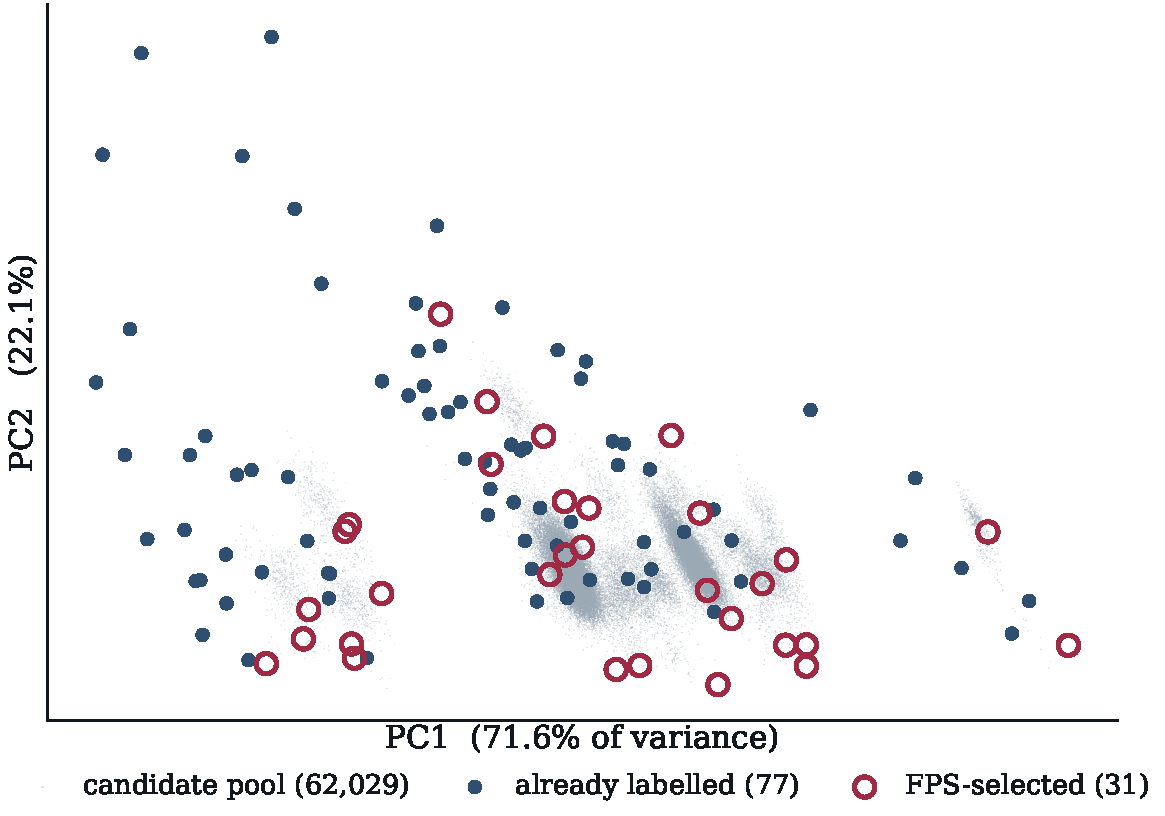
\includegraphics[width=\linewidth]{fig_latent.pdf}
\end{column}
\begin{column}{0.44\textwidth}
\figcap{PC1\,$\times$\,PC2 of L2-normalised 256-d latents, 93.7\% of variance,
from the real it5\,$\rightarrow$\,it6 round. The seed fills the dense core; every
pick lands on the sparse rim --- exactly where the model has never been.}
\vskip0.5em
In the final round $\rho$ collapses $0.0510\rightarrow0.0207$ past
$d_{99}=0.0208$, driving a \textbf{62{,}029-frame pool} from
\wintext{98.999\%\,$\rightarrow$\,100\% coverage} with \goldtext{31 labels}.
\end{column}
\end{columns}
\end{block}

\begin{block}{LoRA: new physics, nothing forgotten}
\begin{columns}[t]
\begin{column}{0.52\textwidth}
The pretrained weights stay \textbf{frozen}. LoRA learns a low-rank correction
that starts at exactly zero:
\begin{equation*}
W_{\mathrm{eff}} = W_0 + \tfrac{\alpha}{r}BA, \qquad r \ll d
\end{equation*}
confining every update to a low-dimensional, task-specific subspace. The model
\textbf{begins from its pretrained state and learns only what is new} --- so the
bulk chemistry it already knows survives the campaign intact.
\end{column}
\begin{column}{0.44\textwidth}
\begin{exampleblock}{Configuration}
\centering
\begin{tabular}{lr}
\toprule
rank $r$ / $\alpha$      & 5 / 1 \\
trainable parameters     & \wintext{$<$1\%} \\
foundation               & mace-omat-0-medium \\
epochs (SWA from 1000)   & 1500 \\
\bottomrule
\end{tabular}
\end{exampleblock}
\end{column}
\end{columns}
\vskip0.4em
{\small Every iteration fine-tunes \textbf{the foundation model afresh}, never
the previous iteration --- so nothing compounds across rounds and each result
stands on its own.}
\end{block}

\end{column}

%% ======================= COLUMN 2 =======================================
\begin{column}{0.465\paperwidth}

\begin{block}{DFT-FE: the engine that makes all of this possible}
\textbf{Every label in this work is a DFT-FE calculation, and the campaign
simply could not be run on any other reference method.} DFT-FE solves
Kohn--Sham DFT in \textbf{real space} with a systematically improvable
\textbf{finite-element} basis --- massively parallel, GPU-accelerated, and the
code behind the \goldtext{2023 ACM Gordon Bell Prize}. Two of its capabilities
are what this entire pipeline rests on.
\vskip0.6em
\begin{columns}[t]
\begin{column}{0.52\textwidth}
\begin{exampleblock}{1. Semi-periodic boundary conditions}
A finite-element basis is local, so periodicity is a \emph{choice per
direction}, not a requirement. DFT-FE runs
\texttt{pbc=[True,True,False]} --- \wintext{periodic in $x,y$, genuinely open
along $z$}.
\vskip0.3em
A plane-wave basis cannot do this at all: 3D periodicity forces an asymmetric
Li\,$|$\,LLZO slab into a \badtext{sandwich} --- a second spurious interface and
an image dipole --- or into a dipole-corrected compromise.
\vskip0.3em
With DFT-FE, every training cell holds \wintext{one real interface and two
genuine free surfaces}: \textbf{the thing that actually exists.}
\end{exampleblock}
\end{column}
\begin{column}{0.46\textwidth}
\begin{exampleblock}{2. Scale}
Real-space domain decomposition scales to cells far beyond plane-wave reach.
Every one of the \goldtext{108} labels is a full ground-state calculation on
\wintext{420--1378 atoms}.
\vskip0.3em
So the potential is \wintext{trained at the size it is deployed} --- no
extrapolation from small periodic approximants up to production MD.
\vskip0.3em
{\small OLCF Frontier, 64 nodes $\times$ 4 MI250X GPUs, one MPI task per GPU.}
\end{exampleblock}
\vskip0.3em
\centering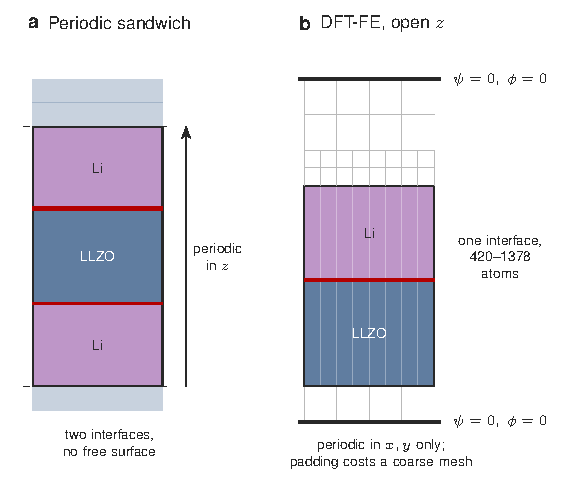
\includegraphics[width=0.96\linewidth]{fig_schematic.pdf}
\end{column}
\end{columns}
\vskip0.5em
\begin{center}\large
\goldtext{Open boundaries fix \emph{what} is modelled; scale fixes \emph{how
big}. DFT-FE delivers both --- and only then does the rest of this pipeline
mean anything.}
\end{center}
\vskip0.4em
{\small\textbf{Setup:} GGA--PBE \textbullet\ SPMS pseudopotentials \textbullet\
FE order 7 \textbullet\ mesh 1.2\,\AA\ \textbullet\ refinement radius 8\,\AA\
\textbullet\ smearing 500\,K \textbullet\ SCF $5\times10^{-5}$\,Ha \textbullet\
zero Dirichlet in $z$.}
\end{block}

\begin{block}{Accuracy: better every single round}
\begin{columns}[t]
\begin{column}{0.46\textwidth}
\centering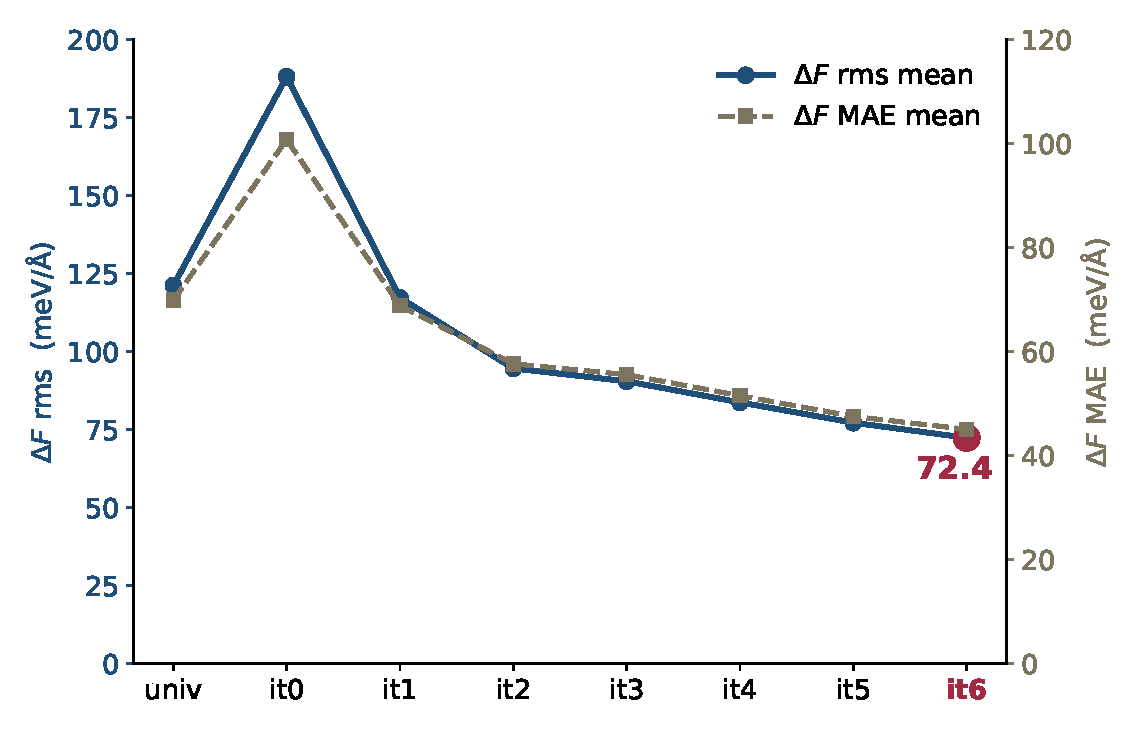
\includegraphics[width=\linewidth]{fig_error.pdf}
\end{column}
\begin{column}{0.51\textwidth}
\centering\small
\begin{tabular}{lrrrr}
\toprule
\textbf{model} & \multicolumn{2}{c}{$\Delta F$ rms}
               & \multicolumn{2}{c}{$\Delta F$ max-comp}\\
\cmidrule(lr){2-3}\cmidrule(lr){4-5}
 & mean & max & mean & max\\
\midrule
foundation & \badtext{121.2} & 201.9 & \badtext{792.3} & 1665.9\\
it0 & 188.1 & 330.4 & 1320.6 & 2472.6\\
it1 & 117.2 & 167.8 &  767.4 & 1239.5\\
it2 &  94.6 & 163.7 &  640.3 & 1190.3\\
it3 &  90.5 & 158.2 &  612.4 & 1111.7\\
it4 &  83.7 & 128.9 &  574.5 &  914.5\\
it5 &  77.2 & 112.9 &  516.2 &  900.1\\
\midrule
\textbf{it6} & \wintext{72.4} & \wintext{99.9} & \wintext{485.2} & \wintext{746.8}\\
\bottomrule
\end{tabular}
\end{column}
\end{columns}
\vskip0.6em
\begin{columns}[t]
\begin{column}{0.48\textwidth}
\begin{exampleblock}{Forces: monotone improvement}
Every round beats the one before it, with \textbf{no plateau in sight}. The
worst single component anywhere --- what actually governs MD stability --- falls
\wintext{1321\,$\rightarrow$\,485 meV/\AA} across the campaign. The final step
alone is significant at \wintext{$p=0.008$}, better on 24 of 33 structures.
\end{exampleblock}
\end{column}
\begin{column}{0.48\textwidth}
\begin{exampleblock}{Energy: locked in early}
Energy reaches \wintext{$\sim$4 meV/atom by it2} and \textbf{holds there through
every later round} --- chemical accuracy achieved early and never given back,
leaving the whole remaining budget free to drive forces down.
\end{exampleblock}
\end{column}
\end{columns}
\vskip0.3em
{\small 33-structure in-domain held-out set, all independent DFT-FE single-point
calculations, component-wise errors in meV/\AA.}
\end{block}

\begin{block}{108 labels, 73{,}634 environments}
\begin{columns}[t]
\begin{column}{0.46\textwidth}
\centering\large
\begin{tabular}{lr}
\toprule
configurations screened   & 414{,}019 \\
\textbf{DFT-FE labelled}  & \goldtext{108} \\
local environments        & \wintext{73{,}634} \\
in-domain held out        & 33 \\
cells, atoms              & 420--1378 \\
\bottomrule
\end{tabular}
\vskip0.6em
\figcap{MACE sees each atom inside its cutoff sphere, so \textbf{every atom in a
labelled cell is a training example}. 108 structures buy 73{,}634 local
environments --- a \textbf{680$\times$} multiplier on the DFT budget.}
\end{column}
\begin{column}{0.51\textwidth}
\centering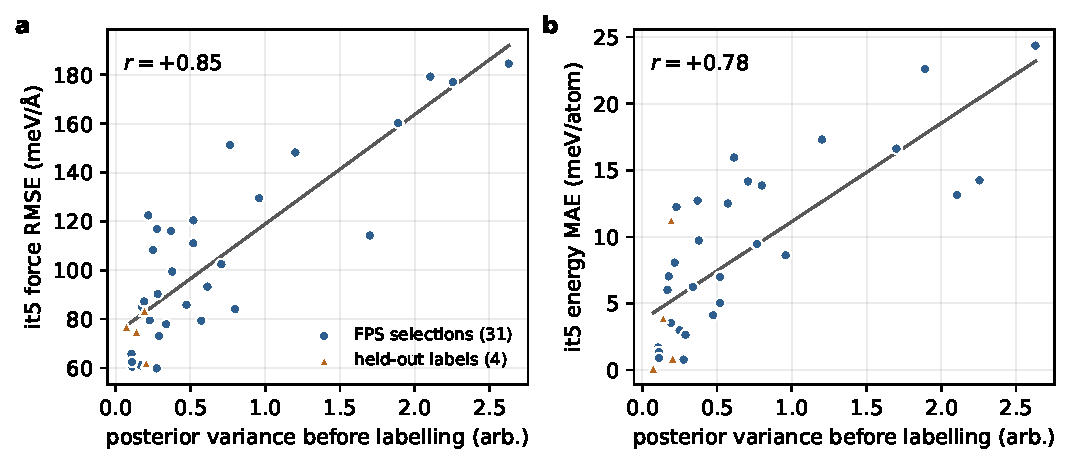
\includegraphics[width=0.95\linewidth]{fig_uq.pdf}
\figcap{A Gaussian-process posterior variance computed in the latent space
\textbf{before} the final round --- available at selection time --- predicts the
error later measured against DFT-FE.}
\end{column}
\end{columns}
\vskip0.5em
\begin{exampleblock}{The acquisition rule is proven, not assumed}
\wintext{$r=+0.85$} on forces, $+0.78$ on energy. It survives leave-one-out
($[+0.82,+0.87]$), bootstrap (95\% CI $[+0.69,+0.93]$) and control for structure
size, and the selected set \wintext{beat all 1000} random subsets of equal size.
The method \textbf{spends the DFT-FE budget exactly where the model is wrong ---
without ever measuring the error.}
\end{exampleblock}
\end{block}

\begin{block}{What this establishes}
\begin{enumerate}
  \item \goldtext{Coverage-driven latent selection} closes a 62{,}029-frame pool
        to \textbf{100\%} with 31 labels, and provably never re-labels a
        near-duplicate.
  \item \goldtext{DFT-FE is the enabler.} Real-space finite elements give
        \textbf{semi-periodic boundary conditions} --- impossible in a
        plane-wave basis --- and ground states on \textbf{420--1378-atom}
        cells. One real interface, two free surfaces, trained at the scale it
        is deployed. \textbf{Remove DFT-FE and the campaign does not exist.}
  \item \goldtext{LoRA} ($r=5$, $<$1\% parameters) absorbs all 108 labels with
        the pretrained chemistry left intact.
  \item \goldtext{Force error cut 40\%} against the foundation model
        (121.2\,$\rightarrow$\,72.4 meV/\AA), improving \textbf{every round},
        with energy at chemical accuracy throughout.
  \item \goldtext{The acquisition rule is independently validated}
        ($r=+0.85$) --- this method is \textbf{measured, not asserted}.
\end{enumerate}
\vskip0.4em
{\small Architecture-agnostic: latent FPS, open-boundary real-space labels and
LoRA transfer directly to Li\,$|$\,LPS, Li\,$|$\,LiPON, NaSICON and other
solid-state interfaces.}
\end{block}

\end{column}
\end{columns}
\end{frame}
\end{document}
